In this section, we first describe our proposed parametric navigational method, which comprises two components:
\begin{enumerate}
\item a parametric method for performing interpolation using only a subset of the microphones, where this subset is determined based on estimated source positions (as described in \secref{sec:08_Proposed_Method:Microphone_Validity}), and
%\item a parametric method for excluding microphones from the interpolation calculation based on estimated source positions (described in \secref{sec:08_Proposed_Method:Microphone_Validity}), and
\item a particular two-band implementation of the regularized least-squares interpolation filters (detailed here in \secreftwo{sec:08_Proposed_Method:Reg-LS_Technique}{sec:08_Proposed_Method:Hybrid_Technique}).
\end{enumerate}
Later in this section, we illustrate basic spectral properties of the interpolation filters in \secref{sec:08_Proposed_Method:Azimuth_Dependence} and briefly discuss practical implementation issues in \secref{sec:08_Proposed_Method:Practical_Implementation}.

%%%% Microphone Validity %%%%
\subsection{Source localization and microphone validity}\label{sec:08_Proposed_Method:Microphone_Validity}
As discussed previously, the ambisonics signals provide a valid description of the captured sound field only in a spherical region around the ambisonics microphone that extends up to the nearest source or obstacle.
Consequently, in order to determine the set of microphones for which the listening position is valid, we must first locate any near-field sources.
Several existing methods for acoustically localizing near-field sources using ambisonics signals from one or more ambisonics microphones are discussed by~\citet[chapter 3]{Zheng2013PhD}, and require only knowledge of the positions and orientations of the microphones.%\footnote{Note that in the present method, we only aim to determine the locations of sources, whereas \citet{Zheng2013PhD} additionally attempts to isolate their emitted signals.}

Briefly, such methods often involve taking a short-time Fourier transform of the first-order ambisonics signals and, for each time-frequency bin, calculating the acoustic intensity vector, as given in \eqnref{eq:04_Auditory_Models:Intensity_Vector}. % \citet[Eq.~(11)]{MerimaaPulkki2005}.
For each ambisonics microphone, a histogram is generated using the direction of the intensity vector at each time and frequency.
The peaks of the histogram indicate source directions, and source positions are determined through triangulation with multiple ambisonics microphones.

Once the locations of the near-field sources are determined, we compare the distances from each microphone to its nearest source and the distance of that microphone to the desired listening position.
Only the signals from those microphones that are nearer to the listening position than to any near-field source are included in the navigation calculation (i.e., all microphones such that $r_p = \|\vec{r}_0 - \vec{u}_p\| < \|\vec{s}_0 - \vec{u}_p\| = s_p$).
A matrix of interpolation filters, described in the following sections, is then computed for and applied to the signals from the remaining ``valid'' microphones.
This procedure is illustrated by the flowchart in \figref{fig:08_Proposed_Method:Flowchart}.

% Flowchart
\begin{figure*}[t]
    \centering
    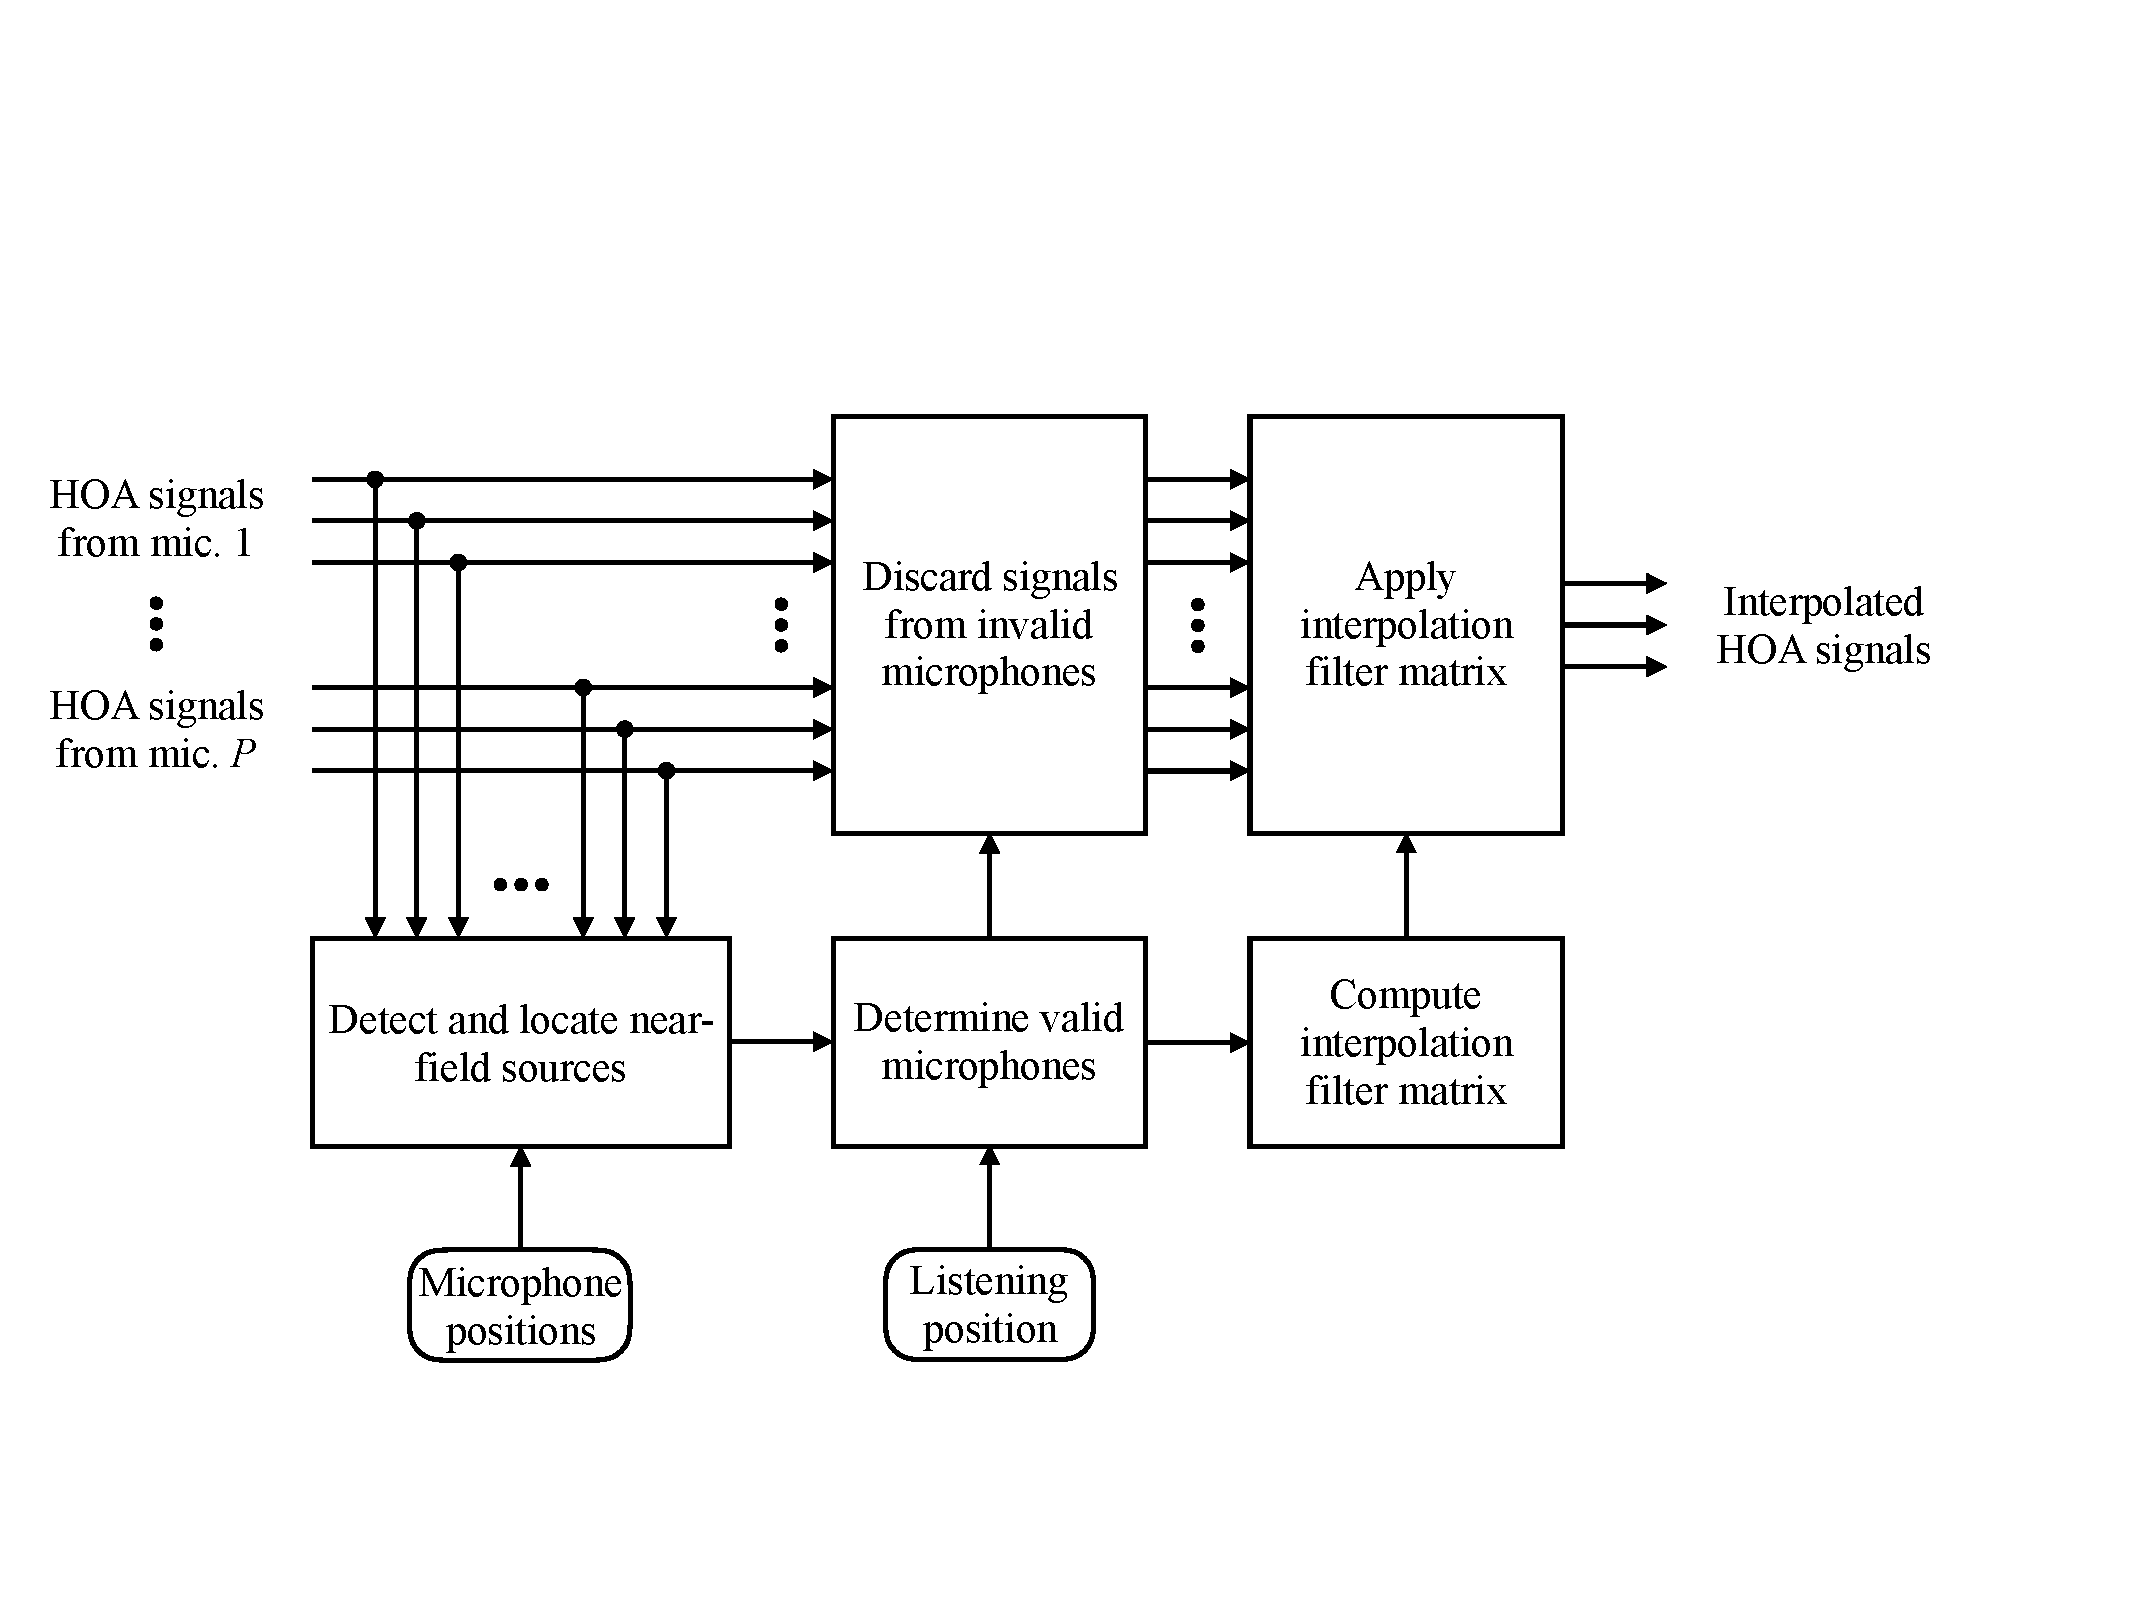
\includegraphics[width = \textwidth,trim={0 4cm 3cm 7cm},clip]{08_proposed_method/figures/Interpolation_Flowchart.pdf}
\caption[Flowchart of the proposed parametric interpolation method.]{
Flowchart of the proposed method for virtual sound field navigation excluding invalid microphones.}
\label{fig:08_Proposed_Method:Flowchart}
\end{figure*}
%%NOTE%% convert to tikz

In this work, we assume that any near-field sound sources can be located accurately and we choose to focus on characterizing the performance of the proposed navigational method under that assumption.
Accordingly, we do not concern ourselves with the sensitivity of the proposed method to inaccuracies in the estimated positions of near-field sources.
This assumption will be valid in scenarios where the positions of the nearest sound sources are either known \textit{a priori} or can be accurately obtained (e.g., through physical distance measurements) \textit{a posteriori}.

%%%% Least-Squares Interpolation Filters %%%%
\subsection{Regularized least-squares interpolation filters}\label{sec:08_Proposed_Method:Reg-LS_Technique}
To compute the interpolation filters, we modify the pseudoinverse-based interpolation method described in \secref{sec:03_Navigation_Techniques:Pinv_Technique} and propose a particular regularization function.
First, we modify \eqnref{eq:03_Navigation_Techniques:Linear_System_Matrices}, such that the matrices are given by
\begin{equation}\label{eq:08_Proposed_Method:Linear_System_Matrices}
\mathbf{M} = 
    \left[ \begin{array}{c}
    \sqrt{w_1} \left( \mathbf{T}(-\vec{r}_1) \right)^\text{T} \\
    \sqrt{w_2} \left( \mathbf{T}(-\vec{r}_2) \right)^\text{T} \\
    \vdots\\
    \sqrt{w_P} \left( \mathbf{T}(-\vec{r}_P) \right)^\text{T}
    \end{array} \right]
,\quad
\mathbf{y} = 
    \left[ \begin{array}{c}
    \sqrt{w_1} \mathbf{b}_1\\
    \sqrt{w_2} \mathbf{b}_2\\
    \vdots\\
    \sqrt{w_P} \mathbf{b}_P
    \end{array} \right],
\end{equation}
where $w_p$ is the interpolation weight for the $p^\textrm{th}$ microphone and recall that $\vec{r}_p = \vec{r}_0 - \vec{u}_p$ is the position of the listener relative to the $p^\textrm{th}$ microphone.

Next, we compute the singular value decomposition of $\mathbf{M}$, such that $\mathbf{M} = \mathbf{U} \Sigma \mathbf{V}^*$, where $(\cdot)^*$ represents conjugate-transposition.
This allows us to compute a regularized pseudoinverse of $\mathbf{M}$, given by \citep[section 5.1]{Hansen1998}
\begin{equation}
\mathbf{L} = \mathbf{V} \Theta \Sigma^{+} \mathbf{U}^*,
\end{equation}
where $(\cdot)^+$ represents pseudoinversion, and $\Theta$ is a square, diagonal matrix whose elements are given by
\begin{equation}
\Theta_{nn} = \frac{\sigma_n^2}{\sigma_n^2 + \beta},
\end{equation}
where $\sigma_n$ is the $n^\textrm{th}$ singular value of $\mathbf{M}$, with $n \in [1,N_\textrm{max}]$.
(Recall that $N_\textrm{max} = (L_\textrm{max} + 1)^2$ and $L_\textrm{max}$ is defined in \eqnref{eq:03_Navigation_Techniques:Pinv_Interpolation_Lmax}.)
In general, the regularization parameter $\beta$ may be a function of frequency.
Here, we choose the magnitude of a high-shelf filter as the regularization function, given by \citep[section 5.2]{Zolzer2008}
\begin{equation}
\beta(k) = \beta_0 \left| \frac{G_{\pi} i \frac{k}{k_0} + 1}{i \frac{k}{k_0} + G_{\pi}} \right|,
\end{equation}
where $G_{\pi}$ is the amplitude of the high-shelf filter and $k_0$ is its zero-dB crossing, which, for convenience, we take to be the same as that given below in \eqnref{eq:08_Proposed_Method:Hybrid_XO_Freq}.
(In our original publication, we had chosen $k_0 = 1 / \Delta$ for simplicity \citep[Eq.~(17)]{TylkaChoueiri2016}, but we did not consider cases where $P \neq 2$.)
We then let
\begin{equation}
\beta_0 = \frac{1}{\sigma_0} \max_n \sigma_n,
\end{equation}
with some constant $\sigma_0 \gg 1$.
Note that the singular values ($\sigma_n$) of $\mathbf{M}$ are calculated for each frequency, so, in general, $\beta_0$ is also frequency-dependent.
Here, we choose $G_{\pi} = 10^{1.5}$ (i.e., 30~dB) and $\sigma_0 = 1000$.

Finally, we obtain an estimate of $\mathbf{a}$ at each $k$, given by
\begin{equation}
\mathbf{\tilde{a}}(k) = \mathbf{L}(k) \cdot \mathbf{y}(k).
\end{equation}
Note that, as with the weighted average method, we may choose to drop the higher-order terms in $\mathbf{\tilde{a}}$ such that we keep only up to order $L_\textrm{out}$, where $L_\textrm{out} \leq L_\textrm{max}$.

Also note that we can factor out the interpolation weights into a diagonal matrix, such that
\begin{equation}
\mathbf{\tilde{a}}(k) = \left( \mathbf{L}(k) \cdot
    \left[ \begin{array}{c c c c}
    \sqrt{w_1}\, \mathbf{I} & \mathbf{0} & \cdots & \mathbf{0}\\
    \mathbf{0} & \sqrt{w_2}\, \mathbf{I} & \ddots & \vdots\\
    \vdots & \ddots & \ddots & \mathbf{0}\\
    \mathbf{0} & \cdots & \mathbf{0} & \sqrt{w_P}\, \mathbf{I}
    \end{array} \right]
 \right) \cdot
     \left[ \begin{array}{c}
    \mathbf{b}_1(k)\\
    \mathbf{b}_2(k)\\
    \vdots\\
    \mathbf{b}_P(k)
    \end{array} \right],
\end{equation}
where $\mathbf{0}$ is an $N_\textrm{in} \times N_\textrm{in}$ matrix of zeros, and $\mathbf{I}$ is the $N_\textrm{in} \times N_\textrm{in}$ identity matrix.
For compactness, we let
\begin{equation}
\mathbf{L}_w(k) = \mathbf{L}(k) \cdot
    \left[ \begin{array}{c c c c}
    \sqrt{w_1}\, \mathbf{I} & \mathbf{0} & \cdots & \mathbf{0}\\
    \mathbf{0} & \sqrt{w_2}\, \mathbf{I} & \ddots & \vdots\\
    \vdots & \ddots & \ddots & \mathbf{0}\\
    \mathbf{0} & \cdots & \mathbf{0} & \sqrt{w_P}\, \mathbf{I}
    \end{array} \right].
\end{equation}

%%%% Hybrid Filters %%%%
\subsection{Two-band interpolation filters}\label{sec:08_Proposed_Method:Hybrid_Technique}
As found in a previous analysis, the regularized least-squares interpolation filters derived in the previous section can induce significant spectral coloration at high frequencies, whereas, below some critical frequency, they induce negligible coloration \citep[cf.~Fig.~4b]{TylkaChoueiri2016}.
%In particular, in the case of $P = 2$ microphones, this critical frequency was found to correspond to $k \Delta \approx 2 L_\textrm{in}$ \citep[cf.~Fig.~5]{TylkaChoueiri2016}.
Consequently, we propose a two-band approach which applies the regularized least-squares interpolation filters at low frequencies ($k < k_0$) and employs the weighted average method at higher frequencies ($k \geq k_0$).
Here, we let
\begin{equation}\label{eq:08_Proposed_Method:Hybrid_XO_Freq}
k_0 = \left\{
  \begin{array}{c l}
  \displaystyle \frac{1}{r_1}, & \text{for } P = 1,\\[8pt]
  \displaystyle \frac{\Delta}{r_1 r_2}, & \text{for } P = 2,\\[8pt]
  \displaystyle \frac{1}{\max_{p\in[1,P]} r_p}, & \text{otherwise},
  \end{array} \right.
\end{equation}
which we found empirically to perform well in terms of coloration.

We then rewrite the weighted average calculation, given in \eqnref{eq:03_Navigation_Techniques:Crossfading}, as a matrix equation, such that
\begin{equation}
\mathbf{\tilde{a}}(k) = 
    \left[ \begin{array}{c c c c}
    w_1 \mathbf{I} & w_2 \mathbf{I} & \cdots & w_P \mathbf{I}
    \end{array} \right]
\cdot
     \left[ \begin{array}{c}
    \mathbf{b}_1(k)\\
    \mathbf{b}_2(k)\\
    \vdots\\
    \mathbf{b}_P(k)
    \end{array} \right],
\end{equation}
where now $\mathbf{I}$ is the $N_\textrm{out} \times N_\textrm{in}$ identity matrix. %%NOTE%% num rows could be N_in, N_max, or N_out
Thus, we define the combined interpolation filter matrix as
\begin{equation}\label{eq:08_Proposed_Method:HybridFilters}
\mathbf{H}(k) = \left\{
  \begin{array}{c l}
  \mathbf{L}_w(k), & \textrm{for } k < k_0, \\
  \left[
    \begin{array}{c c c c}
    w_1 \mathbf{I} & w_2 \mathbf{I} & \cdots & w_P \mathbf{I}
    \end{array}
  \right], & \textrm{for } k \geq k_0.
  \end{array} \right.
\end{equation}
Note that if we have only $P = 1$ valid microphone, the high-frequency filter matrix becomes the identity matrix (since $w_1 = 1$ after normalization).

Given the well-established rule of thumb that a sound field is accurately represented up to a distance $r$ provided that $k r \leq L_\textrm{in}$ \citep{WardAbhayapala2001}, we expect that for $P = 1$, the coloration should be negligible below $k r_1 \approx L_\textrm{in}$.
Additionally, for $P = 2$ microphones, we previously found that coloration appeared negligible below $k \Delta \approx 2 L_\textrm{in}$ for a listener equidistant from the microphones \citep[cf.~Fig.~5]{TylkaChoueiri2016}.
However, these approximations were found to break down due to the near-field compensation filters needed in practice (described in \secref{sec:02_Acoustical_Theory:Ambisonics_Encoding}).
Consequently, here we take a more conservative critical frequency, as in \eqnref{eq:08_Proposed_Method:Hybrid_XO_Freq}.%
\footnote{Note that in this work we do not explore the case of $P > 2$, so a superior critical frequency likely exists.
It may also still be worth pursuing order-dependent critical frequencies for $P = 1,2$, since, in principle, increasing the expansion order should improve accuracy, but we do not do so here.}

%%%% Source Azimuth Dependence %%%%
\subsection{Source azimuth dependence}\label{sec:08_Proposed_Method:Azimuth_Dependence}
In this section, we examine the effective frequency responses induced by translation via the regularized least-squares and hybrid interpolation filters as a function of source azimuth.
As described in \secref{sec:06_Simulation_Framework:Azimuth_Dependence}, for these simulations, we let $L_\text{in} = 4$, pick $\Delta = 0.5$~m and $s_0 = 2.5$~m (so $\gamma = 10$), and interpolate to $\vec{r}_0 = (0, 0, 0)$.
(Recall that these quantities are defined in \secref{sec:06_Simulation_Framework:Linear_Geometry} for a linear array geometry.)

The induced frequency responses are plotted in \figref{fig:08_Proposed_Method:Azimuth_Dependence}.
For the regularized least-squares interpolation filters (see \figref{fig:08_Proposed_Method:Azimuth_Dependence:Pinv}), we see that the frequency response is largely flat below a critical frequency (cf.~\citet[Fig.~4b]{TylkaChoueiri2016}), whereas above that frequency, the response exhibits significant broadband deviations (e.g., for $\varphi_0 = 75^\circ, 90^\circ$) as well as sporadic notches.
Based on well-established psychoacoustic findings, we can expect these distortions to be more audible (that is, either more likely to be audible or more significantly distorted) than the comb-filtering response of the weighted average method \citep{Bucklein1981,Kates1984,Brunner2007}.%
\footnote{In particular, \citet{Bucklein1981} showed that spectral peaks are more audible than notches of the same width and height, and that broadband spectral features are more audible than narrow ones.
Additionally, psychoacoustic studies have shown that comb-filter responses can be imperceptible if the time-delay between the primary and secondary signals is long enough and/or if their relative levels are different enough \citep{Kates1984,Brunner2007}.}

\begin{figure*}[t]
    	\centering
    	\begin{subfigure}[b]{0.49\textwidth}
        		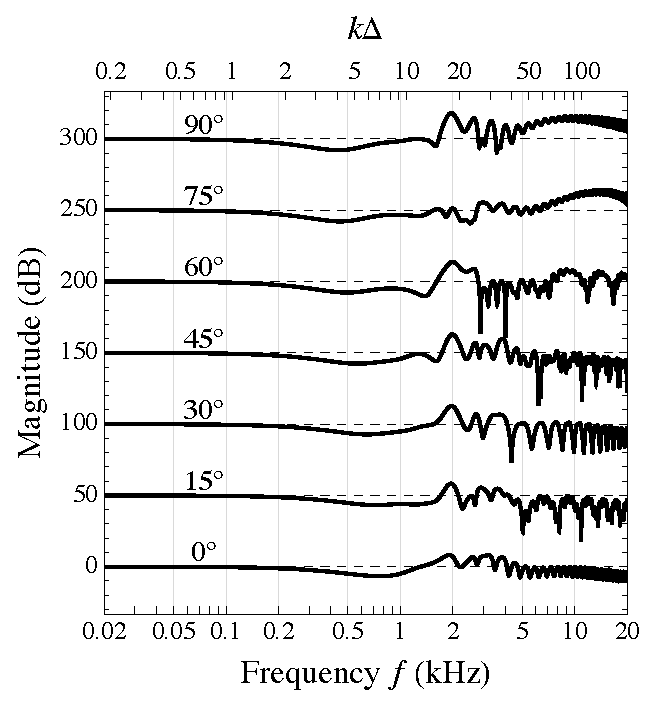
\includegraphics[width=\textwidth]{08_proposed_method/figures/sourceAz_freqResp_pinv.eps}
        		\caption{Regularized least-squares filters}
        		\label{fig:08_Proposed_Method:Azimuth_Dependence:Pinv}
    	\end{subfigure}
	\hfill
    	\begin{subfigure}[b]{0.49\textwidth}
        		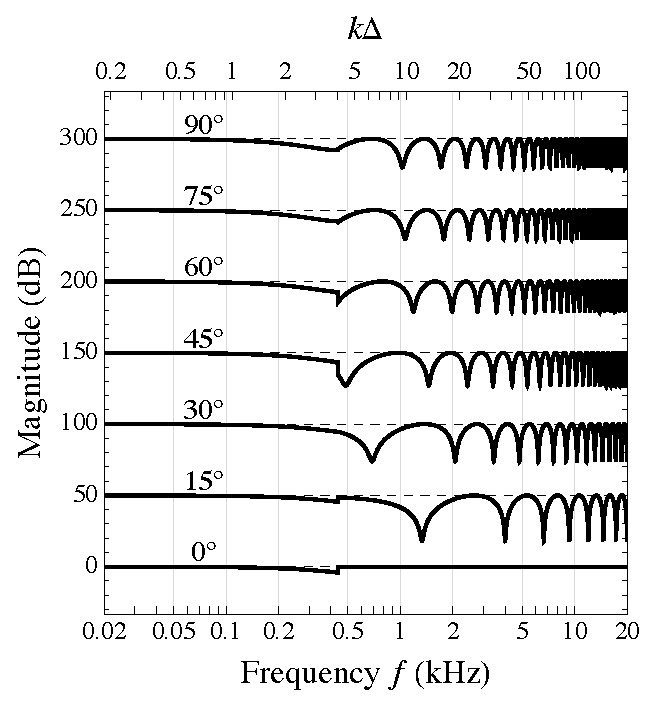
\includegraphics[width=\textwidth]{08_proposed_method/figures/sourceAz_freqResp_validhybrid.eps}
        		\caption{Hybrid filters}
        		\label{fig:08_Proposed_Method:Azimuth_Dependence:Hybrid}
    	\end{subfigure}
	
	\caption[Magnitude responses across azimuths for each interpolation filter.]{
	Magnitude responses caused by the regularized least-squares and hybrid interpolation filters for various source azimuths.
  The bottom axes show frequency in kHz while the top axes show the nondimensional frequency $k\Delta$ for a microphone spacing of $\Delta = 0.5$~m.
  For legibility, each frequency response is offset by $50$~dB and the responses have been artificially truncated (where needed) to not exceed $-45$~dB.}
	\label{fig:08_Proposed_Method:Azimuth_Dependence}
\end{figure*} %%NOTE%% vertical axis label is too complicated: |A0 / B0ref| or something

As shown in \figref{fig:08_Proposed_Method:Azimuth_Dependence:Hybrid}, the hybrid filters exhibit precisely this comb-filtering frequency response above the critical frequency, $k_0$, given in \eqnref{eq:08_Proposed_Method:Hybrid_XO_Freq}.
Below this critical frequency, however, the hybrid filter responses exhibit a wide, flat region, rather than the continued comb-filtering response exhibited by the weighted average method (as shown in \figref{fig:08_Proposed_Method:XF_CombFiltering}).
Consequently, we expect the coloration incurred by the hybrid filters to be less severe than that incurred by the weighted average method.

%%%% Practical Implementation %%%%
\subsection{Practical implementation}\label{sec:08_Proposed_Method:Practical_Implementation}
In practice, as the listener traverses the navigable region, the number of valid microphones may change.
Consequently, one should crossfade between audio frames to prevent any audible discontinuities caused by a sudden change in the filters.
Additionally, it is likely preferable to implement a ``crossover'' between the low- and high-frequency ranges of the combined filter matrix, thereby blending the two filter matrices.
Here, however, we take a simple frequency-domain concatenation approach, as indicated in \eqnref{eq:08_Proposed_Method:HybridFilters}.

%If $\mathbf{M}$ is singular, such that $\mathbf{M}^+$ is undefined, we ``dither'' the weights $w_p$.

Although in this work we only consider interpolation to points within the strictly-interior navigable region (i.e., the area spanned by the microphone array), navigation outside of this region may be achieved in practice through a two-stage navigation approach.
In such an approach, the recorded signals are first interpolated to the point within the strictly-interior region nearest to the desired listening position.
Then, those interpolated signals are effectively treated as a new virtual ambisonics microphone and extrapolated to the desired listening position.